\section{Reproduction Using TabPFN-Derived Datasets}
\label{sec:transformed-reproduction}

\subsection{Purpose and evaluation designs}

Section~\ref{sec:transformations} introduced two distinct transformations of the
clinical data.  The embedding transformation represents each original patient by
dense numerical coordinates learned by a Tabular Prior-Data Fitted Network
(TabPFN).  Synthetic generation instead produces new records containing clinical
predictors and outcomes in the same format as the original cohort.  This section
examines whether the diagnostic and prognostic modelling procedures can be applied
to both transformed datasets and how much predictive structure they retain.

These analyses do not constitute external validation.  The embedding models are
evaluated on the original patients, and the synthetic models are evaluated only on
generated records.  They also do not test synthetic augmentation, because no
synthetic records are added to a real-data training set in this section.

Table~\ref{tab:transformed:contracts} summarises the four evaluation designs.
Out-of-fold (OOF) predictions are predictions for patients who were excluded from
the downstream model fit that produced their prediction.  For the embedding
analyses, however, the TabPFN representations had already been constructed using
the full cohort.  The downstream OOF or training-validation procedures therefore
reduce overfitting in the prediction model but do not provide a fully separated
evaluation of the complete transformation-and-modelling process.

\begin{table}[htbp]
\centering\small
\caption{Evaluation designs used for the TabPFN-derived datasets.}
\label{tab:transformed:contracts}
\begin{tabularx}{\linewidth}{@{}>{\RaggedRight\arraybackslash}p{2.0cm}
>{\RaggedRight\arraybackslash}p{1.45cm}YY@{}}
\toprule
Dataset & Task & Model and evaluation & Interpretation \\
\midrule
Real-patient embeddings & Diagnosis & Ridge logistic regression on 512
coordinates; 10-fold OOF downstream predictions for all 2,672 patients &
Exploratory internal evaluation because the embeddings were created before the
downstream folds \\
Real-patient embeddings & Prognosis & Ridge Cox model on 1,024 coordinates;
trained on 323 patients and evaluated on 139 patients & Exploratory internal
validation because the embeddings were created before the 323/139 split \\
Synthetic cohort & Diagnosis & Clinical logistic models fitted and evaluated on
all 3,000 generated records & Fitted-cohort performance; no independent test set \\
Synthetic cohort & Prognosis & Clinical Cox models trained on 323 generated
records and evaluated on 139 generated records & Internal validation within the
generated cohort; no evaluation on real patients \\
\bottomrule
\end{tabularx}
\end{table}
\FloatBarrier

\subsection{Performance summary across data sources}

Tables~\ref{tab:transformed:diagnostic-summary} and
\ref{tab:transformed:prognostic-summary} bring together the main results from
the published study, the SEER reproduction, the independent UK Erlangen
evaluation and the TabPFN-derived datasets. They provide a compact overview,
but they are not a single model ranking. The published values come from a
different patient cohort; the diagnostic SEER and complete-synthetic results
were calculated in the same records used for model fitting; the Erlangen
results are external; and the embedding results use held-out downstream
predictions even though the representations were created from the complete
cohort. Direct comparisons are therefore most reliable within rows that share
the same data and evaluation procedure.

\begin{table}[htbp]
\centering\scriptsize
\setlength{\tabcolsep}{3pt}
\caption{Compact diagnostic performance summary. ROC AUC is the area under the
receiver operating characteristic curve; brackets give the 95\% confidence
interval. Published values are from \citet{Li2023}. The data-type column
distinguishes evaluations using clinical records, TabPFN embeddings or fully
synthetic records.}
\label{tab:transformed:diagnostic-summary}
\begin{tabularx}{\linewidth}{@{}p{2.05cm}p{1.50cm}p{2.35cm}r
>{\RaggedLeft\arraybackslash}p{2.35cm}Y@{}}
\toprule
Data and evaluation & Data type & Model & $n$ & ROC AUC [95\% CI] & Meaning of the estimate \\
\midrule
\csname @@input\endcsname{tables/transformed_reproduction/cross_section_diagnostic_rows.tex}
\bottomrule
\end{tabularx}
\end{table}

\begin{table}[htbp]
\centering\scriptsize
\setlength{\tabcolsep}{3pt}
\caption{Compact prognostic performance summary. Harrell C is Harrell's
concordance index, and the remaining columns give time-dependent AUC at 12, 24
and 36 months. The data-type column distinguishes evaluations using clinical
records, TabPFN embeddings or fully synthetic records. Published values are
from \citet{Li2023}. For the synthetic rows, concordance is calculated in the
323-record training subset and AUC in the 139-record generated validation
subset. AIC denotes Akaike information criterion; RF/RFE denotes random-forest
recursive feature elimination. A dash indicates that the corresponding value
was not reported.}
\label{tab:transformed:prognostic-summary}
\begin{tabularx}{\linewidth}{@{}p{2.35cm}p{1.50cm}Yrrrr@{}}
\toprule
Data and evaluation & Data type & Model & Harrell C & AUC 12 m & AUC 24 m & AUC 36 m \\
\midrule
\csname @@input\endcsname{tables/transformed_reproduction/cross_section_prognostic_rows.tex}
\bottomrule
\end{tabularx}
\end{table}
\FloatBarrier

\subsection{Origin and interpretation of the clinical T/N comparators}
\label{sec:transformed:tn-comparator}

The American Joint Committee on Cancer (AJCC) tumour stage (T) and nodal stage
(N) were not included among the embedding coordinates.  The T/N curves shown in
this section come from separate models fitted with these two clinical variables.
For the real-patient embedding analyses, the T and N values belong to the same
SEER patients represented by the embeddings.  All 2,672 diagnostic patients and
all 462 prognostic patients matched one-to-one, with no missing or duplicated
matches.  For the synthetic analyses, the comparator uses the T and N values
generated as part of each synthetic record.

The diagnostic comparison is not symmetric.  The embedding ridge model is
assessed with 10-fold OOF downstream predictions, whereas the clinical pipeline
and the two-variable T/N model are fitted and evaluated on the complete diagnostic
cohort.  Their areas under the receiver operating characteristic curve (AUCs)
should therefore be interpreted as descriptive results under different evaluation
conditions, not as a formal head-to-head model comparison.

For prognosis, the embedding ridge model, the clinical reference model and the
T/N comparator are trained on the same 323 patients and evaluated on the same 139
patients.  This aligns the downstream evaluation sets.  Nevertheless, the
embeddings were constructed before this split, so the validation cohort was not
independent of the representation-learning step.

\subsection{Diagnostic reproduction}

\subsubsection{Real-patient embedding model}

The diagnostic embedding model is a ridge-penalised logistic regression using all
512 embedding coordinates.  Ridge regularisation is suitable for this dense,
correlated representation and avoids selecting individual anonymous coordinates
as if they were clinical variables.  Ten-fold OOF downstream predictions produced
an AUC of 0.900 and a Brier score of 0.0872.  The Brier score is the mean squared
difference between the predicted probabilities and the observed binary outcomes;
lower values indicate smaller probability errors.

Table~\ref{tab:transformed:diag-real} places this result beside the eight-variable
clinical pipeline and the two-variable clinical T/N comparator.  Their AUCs were
0.903 and 0.763, respectively.  Because the two clinical models were fitted and
evaluated on the full cohort, the numerical similarity between the clinical
pipeline and embedding model must not be interpreted as evidence of equivalent
performance.

\begin{table}[htbp]
\centering\small
\caption{Diagnostic discrimination in the 2,672 real SEER patients.  Confidence
intervals condition on the fitted models and the available predictions; they do
not include uncertainty from repeating embedding construction or clinical
variable selection.}
\label{tab:transformed:diag-real}
\begin{tabularx}{\linewidth}{@{}Ycc>{\RaggedRight\arraybackslash}p{2.25cm}@{}}
\toprule
Model and evaluation & Predictors & AUC [95\% CI] & Predictor domain \\
\midrule
\csname @@input\endcsname{tables/transformed_reproduction/diagnostic_real_auc_rows.tex}
\bottomrule
\end{tabularx}
\end{table}

Calibration was summarised by grouping predictions into ten risk groups and
regressing the observed group frequencies on the mean predicted risks.  This gave
an intercept of 0.002 and a slope of 0.986.  These grouped linear-regression values
are not the conventional individual-level logistic calibration intercept and
slope, and therefore do not establish near-perfect calibration.  Calibration was
not calculated for the clinical T/N comparator.

\subsubsection{Synthetic diagnostic cohort}

The clinical feature-selection procedure was repeated in the 3,000-record
synthetic diagnostic cohort.  The least absolute shrinkage and selection operator
(LASSO) retained 15 clinical variables at the minimum-error penalty and five at
the more conservative one-standard-error penalty.  The five variables retained by
the final pipeline were chemotherapy, primary-site surgery, nodal status, tumour
stage and tumour-size group.  This differs from the eight-variable model selected
from the real cohort and indicates that the generated data contain a different
predictor-outcome structure.

\begin{table}[htbp]
\centering\small
\caption{Diagnostic discrimination within the synthetic cohort.  Every model was
fitted and evaluated on the same 3,000 generated records, so the values describe
fitted-cohort performance rather than validation performance.}
\label{tab:transformed:diag-synthetic}
\begin{tabularx}{\linewidth}{@{}Ycc>{\RaggedRight\arraybackslash}p{2.8cm}@{}}
\toprule
Model & Predictors & AUC [95\% CI] & Evaluation \\
\midrule
\csname @@input\endcsname{tables/transformed_reproduction/diagnostic_synthetic_auc_rows.tex}
\bottomrule
\end{tabularx}
\end{table}

The pipeline-selected model had the largest AUC, 0.926.  This value is optimistic
because variable selection, model fitting and evaluation all used the same
synthetic cohort.  Re-estimating calibration on the same fitting data produced an
intercept of zero and slope of one, as expected for an unpenalised logistic model
evaluated on its training data; these values provide no evidence of performance
on new records.

\FloatBarrier
\subsection{Prognostic reproduction}

\subsubsection{Real-patient embedding model}

The prognostic embedding model is a ridge-penalised Cox proportional-hazards model
using 1,024 coordinates: 512 from the death-status embedding and 512 from the
follow-up-time embedding.  The model was fitted on 323 patients and evaluated on
139 patients using the same split as the clinical reference model.  The validation
cohort contained 92 deaths during total follow-up, including 33 by 12 months, 50
by 24 months and 61 by 36 months.

\begin{table}[htbp]
\centering\small
\caption{Time-dependent AUC in the common real-patient validation cohort
(\(n=139\)).  Marginal censoring weights were estimated within the validation
cohort for each calculation.}
\label{tab:transformed:prog-real}
\begin{tabularx}{\linewidth}{@{}cYYYr@{}}
\toprule
Horizon (months) & Clinical reference & Embedding ridge & Clinical T/N comparator & Deaths by horizon \\
\midrule
\csname @@input\endcsname{tables/transformed_reproduction/prognostic_real_validation_auc_rows.tex}
\bottomrule
\end{tabularx}
\end{table}

The embedding model achieved AUCs of 0.861, 0.858 and 0.843 at 12, 24 and 36
months.  The corresponding clinical-reference values were 0.886, 0.873 and
0.844.  The confidence intervals overlap substantially, but the design does not
support claims of equivalence or superiority because the embeddings were created
before the training-validation split.  The clinical T/N comparator performed
poorly, with AUCs of 0.391, 0.443 and 0.505.

The embedding model did not undergo a prognostic calibration analysis.  Its
results therefore support statements about discrimination and risk-group
separation only, not about the accuracy of its predicted survival probabilities.
The follow-up-time embedding also treats observed follow-up as a regression target
without explicitly modelling censoring, which limits its interpretation as a
survival-specific representation.

\subsubsection{Synthetic prognostic cohort}

The 462 generated prognostic records were divided into 323 training records and
139 validation records.  Several Cox model specifications were considered because
they answer different questions.  The primary five-variable model reproduces the
reference study's nomogram specification and contains brain metastasis, age,
histological grade, histological group and primary-site surgery.  Data-driven
alternatives used backward selection by the Akaike information criterion (AIC),
random-forest recursive feature elimination (RF-RFE), or the filtered union of
both selections.  A separate two-variable T/N model provided a simple stage-based
comparator.  The main validation results below use the primary five-variable Cox
model, not the data-driven alternatives.

\begin{table}[htbp]
\centering\small
\caption{Time-dependent AUC in the synthetic validation cohort (\(n=139\)).
Both predictors and outcomes are generated, so this evaluates consistency within
the synthetic cohort rather than transfer to real patients.}
\label{tab:transformed:prog-synthetic}
\begin{tabularx}{\linewidth}{@{}cYYr@{}}
\toprule
Horizon (months) & Primary five-variable Cox model & Synthetic T/N comparator & Deaths by horizon \\
\midrule
\csname @@input\endcsname{tables/transformed_reproduction/prognostic_synthetic_validation_auc_rows.tex}
\bottomrule
\end{tabularx}
\end{table}

The primary model achieved validation AUCs of 0.831, 0.848 and 0.830 at 12, 24
and 36 months.  Its concordance in the synthetic training cohort was 0.706
[0.672--0.741], compared with 0.538 [0.500--0.576] for the synthetic T/N model.
The global proportional-hazards test for the primary model was significant
(\(p=0.0027\)); the surgery and histological-group terms also showed individual
violations.  Its hazard ratios should therefore not be assumed to remain constant
throughout follow-up.  Grade IV was absent from the entire synthetic cohort, so
its association could not be estimated.

Calibration was assessed by grouped observed-versus-predicted regressions in the
synthetic validation cohort.  The slopes were 1.487, 1.323 and 1.226 at 12, 24
and 36 months.  These are descriptive grouped summaries, not conventional
individual-level survival-calibration slopes, and they apply only to this one
generated cohort.

\begin{figure}[htbp]
\centering
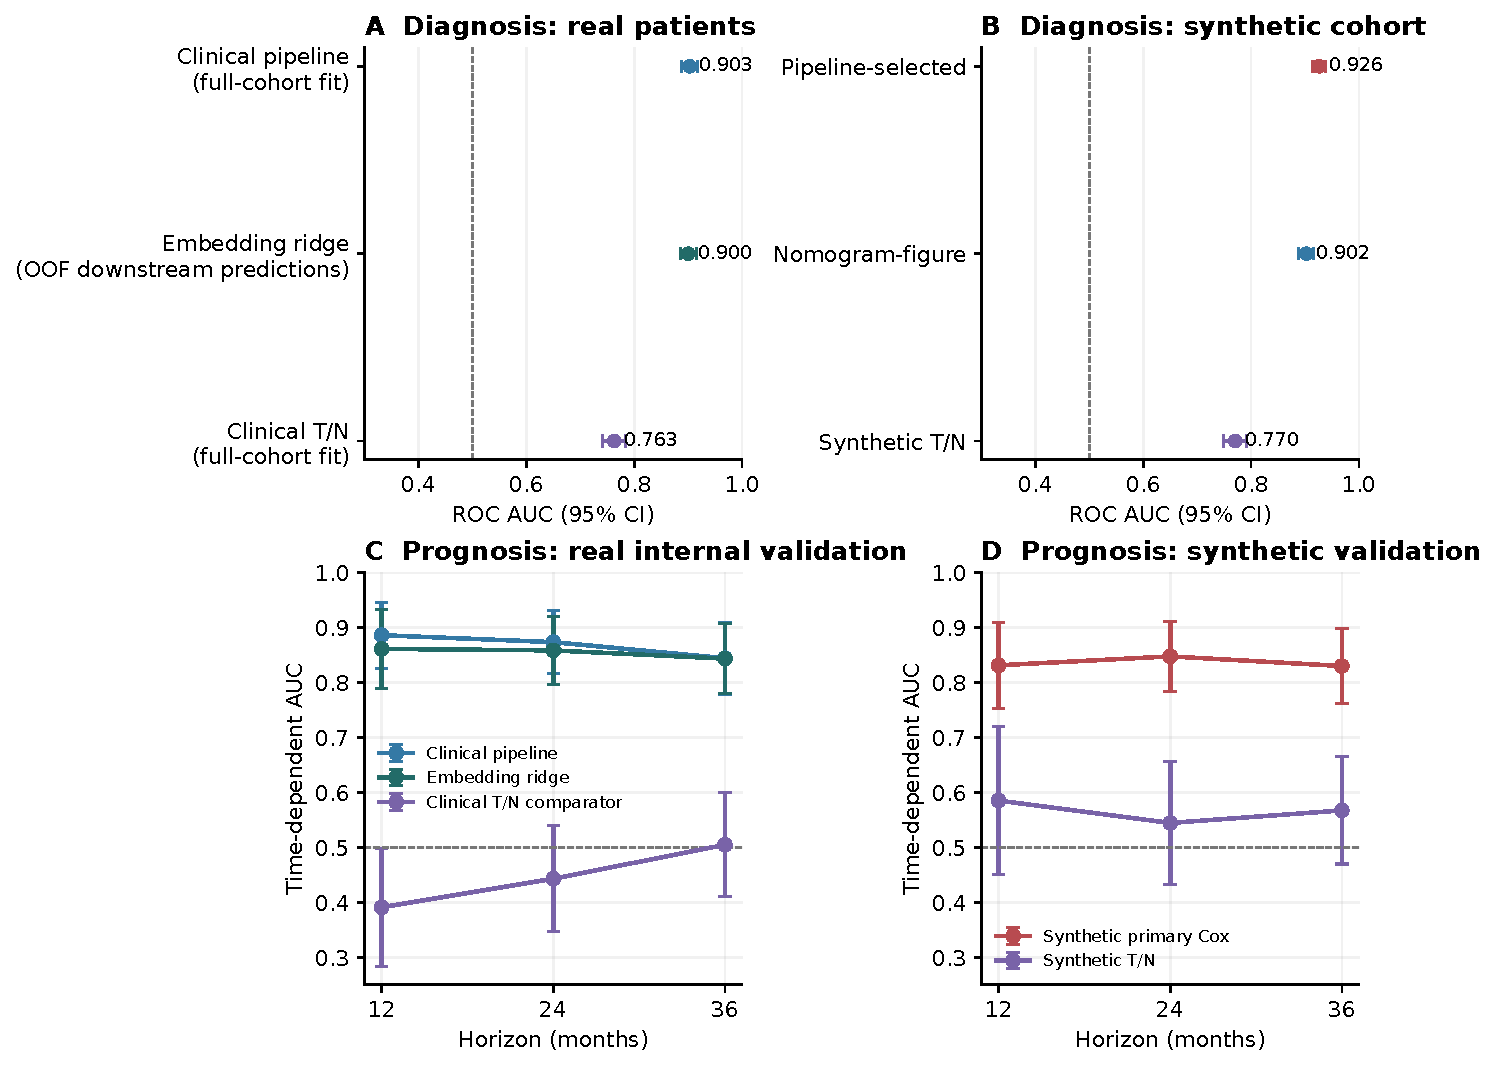
\includegraphics[width=\linewidth]{transformed_reproduction/transformed_auc_overview.pdf}
\caption{Discrimination results separated by data domain and evaluation design.
Panels A and C use real SEER patients; Panels B and D use generated records.  In
Panel A, the embedding model uses downstream out-of-fold predictions while the
clinical models use full-cohort fitted predictions.  In Panel C, the downstream
models share the same validation patients, but embedding construction preceded
the split.  Values in different panels are therefore not directly comparable.}
\label{fig:transformed:auc-overview}
\end{figure}
\FloatBarrier

For risk stratification, each prognostic model used the median linear predictor in
its training cohort as the threshold between low- and high-risk groups.  The same
threshold was then applied unchanged to the corresponding validation cohort.
Table~\ref{tab:transformed:risk-groups} reports the ridge embedding model for the
real patients and the primary five-variable Cox model for the synthetic patients.

\begin{table}[htbp]
\centering\small
\caption{Validation-cohort risk groups for the real-patient embedding ridge model
and the primary five-variable synthetic Cox model.  The two cohorts contain
different records and must not be pooled or compared as if they were one sample.}
\label{tab:transformed:risk-groups}
\begin{tabularx}{\linewidth}{@{}YYrrr@{}}
\toprule
Data and model & Risk group & Patients & Deaths & Median OS (months) \\
\midrule
\csname @@input\endcsname{tables/transformed_reproduction/risk_group_rows.tex}
\bottomrule
\end{tabularx}
\end{table}

Among the real validation patients, median overall survival (OS) was 84 months in
the low-risk group and 18.5 months in the high-risk group.  In the synthetic
validation cohort, the corresponding medians were 94 and 24 months.  These
separations show that each model orders patients or generated records by risk
within its own evaluation domain; they do not show that the synthetic model
transfers to real patients.

\FloatBarrier
\subsection{Decision-curve analysis}

Decision-curve analysis (DCA) expresses the clinical consequences of predictions
as net benefit across a range of decision thresholds.  For diagnosis, net benefit
was calculated for all 2,672 real patients.  The embedding curve uses OOF
downstream predictions, whereas the clinical T/N curve uses probabilities from a
model fitted on the complete cohort.  This asymmetry makes their visual comparison
descriptive rather than confirmatory.

For prognosis, Figure~\ref{fig:transformed:dca} shows the 24-month results in the
139 real validation patients.  Patients censored before a given horizon would be
excluded because their binary outcome at that time is unknown; all 139 patients
were eligible at 24 months.  This complete-case horizon approach does not use
inverse-probability-of-censoring weights and may be biased when censoring is
related to risk.

\begin{figure}[htbp]
\centering
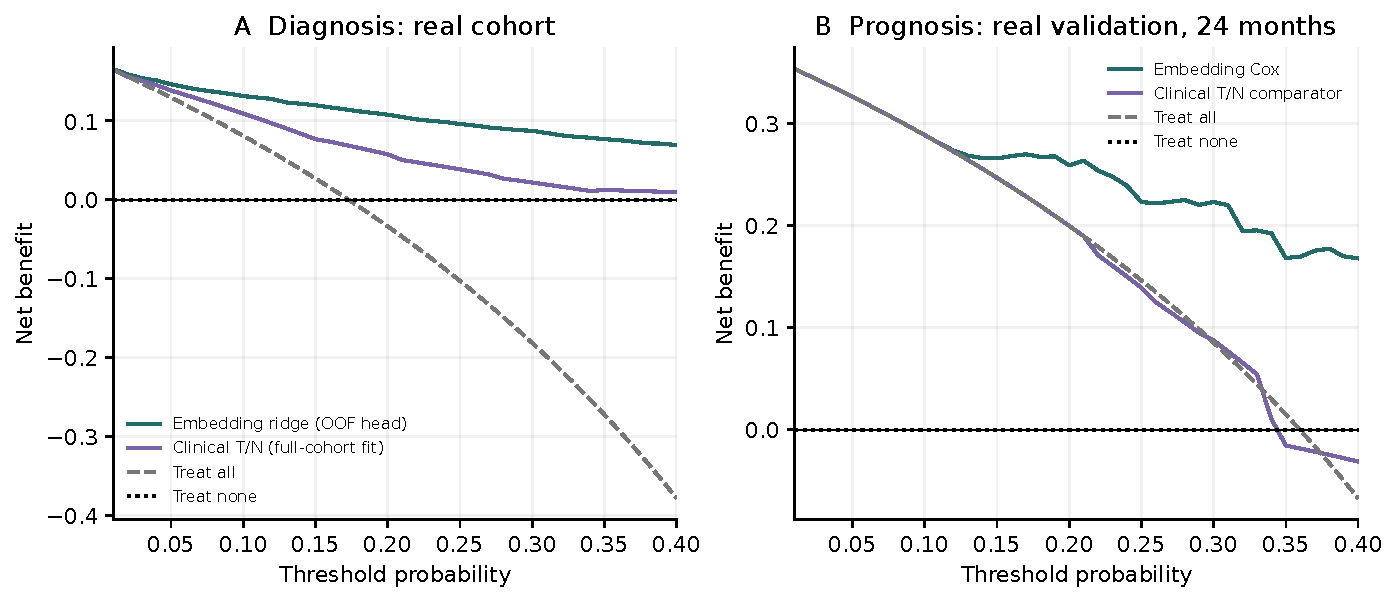
\includegraphics[width=\linewidth]{transformed_reproduction/embedding_dca_clarified.pdf}
\caption{Decision curves for the real-patient embedding models and separate
clinical T/N comparators.  The diagnostic curves use different fitting and
evaluation conditions.  The prognostic curves use the common 139-patient
validation cohort at 24 months and the complete-case horizon approximation.}
\label{fig:transformed:dca}
\end{figure}
\FloatBarrier

No uncertainty intervals for net benefit were calculated, and no clinically
preferred threshold range was specified in advance.  The curves therefore show
how the available predictions behave under the stated net-benefit calculation;
they do not establish clinical usefulness.

\FloatBarrier
\subsection{Interpretation and transition}

The embedding analyses show that regularised prediction models can recover strong
diagnostic and prognostic ordering from the TabPFN coordinates.  The resulting
AUCs are close to those of the clinical reference models, but this is exploratory
evidence.  Full-cohort representation construction, different diagnostic
evaluation procedures and incomplete calibration prevent a confirmatory
comparison.

The synthetic analyses show that the clinical modelling procedures can be
executed on generated cohorts and can recover internally discriminative models.
They do not demonstrate clinical generalisation.  Diagnostic models were fitted
and evaluated on the same generated records, prognostic validation remained
entirely synthetic, and the absence of grade IV patients limits the clinical
support of both generated cohorts.  The changed feature-selection results and the
proportional-hazards violations further show that the synthetic data do not fully
reproduce the structure of the real cohorts.

A stricter embedding comparison would construct each representation using only
the training patients in an outer split, fit the clinical and embedding models
within that split, and compare paired predictions on untouched real test patients.
The following section complements the predictive results presented here by
directly evaluating representation similarity and synthetic-data fidelity.
